% Terra system paper: first draft, Oct 27, 2026.
% IEEE conference format (IEEEtran), target 6--8 pages.
% Facts are transcribed from Terra main 3b8024a, ARGOS main b7064a6, Zorvane main 34f0601
% (all Oct 27, 2026) and from thesis Ch3/Ch5. No result in this draft is invented:
% every measured number has a source in the thesis or the project's experiment folders,
% and everything not yet measured is a \todo{}.
% The sensor evaluation (VIO scale vs OptiTrack, sensor timing, Debug vs Release,
% GNSS, endurance) belongs to the companion phone paper; cite it, do not repeat it.
\documentclass[conference]{IEEEtran}

\usepackage{cite}
\usepackage{amsmath,amssymb}
\usepackage{graphicx}
\usepackage{booktabs}
\usepackage{array}
\usepackage{tabularx}
\usepackage{xcolor}
\usepackage{url}
\usepackage{tikz}
\usetikzlibrary{positioning,arrows.meta,fit,backgrounds}
\usepackage[hidelinks]{hyperref}

\newcommand{\todo}[1]{\textcolor{red}{[TODO: #1]}}

\begin{document}

\title{Terra: A Phone-Brained Rover with a Six-Level Autonomy Ladder, from Teleoperation to On-Device Language-Model Tasking}

\author{\IEEEauthorblockN{Yojan Gautam}
\IEEEauthorblockA{\todo{affiliation, department, university}\\
\todo{email}}}

\maketitle

\begin{abstract}
We present Terra, a ground rover whose only onboard sensor head and computer is a consumer iPhone.
Terra splits the phone software along one rule: a thin Swift layer gathers sensor data (ARKit pose and LiDAR depth, the IMU, GNSS, the camera) and talks to the hardware, while a shared Rust core, about 41{,}000 lines in 17 crates, owns the control loop, safety gating, mapping, planning and every autonomy level.
The same Rust crates run in the Zorvane simulator and are driven from the ARGOS operator dashboard, so one control path is exercised on the phone, in simulation and in the operator's hands.
On this core Terra implements a ladder of six autonomy levels, from L0 teleoperation through assisted driving, direct and obstacle-avoiding waypoints and frontier exploration with object search, to L5, at which an on-device foundation model proposes waypoints for a typed task and the Rust core checks every one before the rover moves.
Three mechanisms make the ladder usable outdoors on a phone: a floor veto that uses ARKit's classified mesh to clear false obstacles from the depth map, a GPS destination accepted at every level from L2 to L5 with a drift-tolerant geographic anchor while the local map still handles obstacles, and a YOLO detector that places buckets and balls on the map with local and geographic coordinates.
We describe the architecture and the design rules that came out of building it, and we propose a field evaluation of the ladder.
\todo{Replace this sentence with the headline field results once Section~\ref{sec:eval} is run.}
\end{abstract}

\begin{IEEEkeywords}
mobile robots, smartphone robotics, levels of autonomy, field robotics, software architecture, on-device language models
\end{IEEEkeywords}

% ---------------------------------------------------------------------------
\section{Introduction}
\label{sec:intro}

A fleet of small rovers that one person can supervise is useful wherever ground has to be covered quickly: search, inspection, and competitions built to rehearse both.
Each rover in such a fleet needs depth sensing, a pose estimate, a radio, a battery and enough compute to plan, and the usual way to get them is a single-board computer cabled to a separate sensor suite.
A current phone already contains all of these in one sealed, mass-produced package, installed by downloading an app.

Earlier phone robots used the phone as a camera and computer for learned driving policies~\cite{muller2021openbot}, or as a sensor and display module on a larger robot~\cite{oros2013smartphone,fong2013smartspheres}.
Terra goes further in one direction: the phone is the rover's \emph{only} sensor head and computer, it carries a full classical autonomy stack, and that stack exposes a graded set of autonomy levels to a remote operator, which is what a supervisory-control study of one operator and many robots needs~\cite{parasuraman2000levels,beer2014lora,goodrich2001adjustable,cummings2008capacity}.

A companion paper asks whether the phone's sensors are good enough, measuring visual--inertial odometry against motion capture, sensor timing and the effect of the build configuration~\cite{companion2026phone}.
This paper asks the systems question: how should the software on a phone-brained rover be structured so that the same autonomy runs on the phone, in simulation and under an operator, and what does each autonomy level need from it?

The contributions are:
\begin{enumerate}
\item An architecture for a phone-brained rover in which a platform layer (Swift on iOS, Kotlin on Android) only bridges sensors and radios, and a shared Rust core owns control, safety, mapping and autonomy, linked unchanged by the simulator (Sections~\ref{sec:arch}--\ref{sec:loop}).
\item A six-level autonomy ladder, L0--L5, built on one arbiter and one local planner, in which every level from L2 up accepts a GPS destination while obstacles stay in the local map, and in which the top level lets an on-device language model choose \emph{where} but never \emph{how} the rover moves (Section~\ref{sec:ladder}).
\item Two phone-specific perception mechanisms: a floor veto from ARKit's classified scene mesh, and a detector-fed object map with geographic coordinates (Sections~\ref{sec:map} and~\ref{sec:objects}).
\item The integration of the rover with an operator dashboard and a competition simulator through one topic contract, and an evaluation design for the whole ladder in the field (Sections~\ref{sec:integration} and~\ref{sec:eval}).
\end{enumerate}

% ---------------------------------------------------------------------------
\section{Related Work}
\label{sec:related}

\paragraph{Phones as robot brains}
OpenBot turned a phone into the brain of a low-cost wheeled robot and trained driving policies on it~\cite{muller2021openbot}.
Smartphone-based robots on the International Space Station used the phone as a sensor and compute payload on a free flyer~\cite{fong2013smartspheres}.
Benchmarks of commercial visual--inertial odometry found ARKit among the most accurate and stable~\cite{kim2022benchmark}, and ARKitScenes shows the phone's LiDAR is good enough for indoor scene reconstruction~\cite{baruch2021arkitscenes}.
None of these systems runs a layered classical stack with operator-selectable autonomy levels on the phone.
\todo{Add two or three recent (2024--2026) phone-robot systems after a literature search; mark each as verified.}

\paragraph{Field autonomy stacks}
Team CERBERUS in the DARPA Subterranean Challenge ran exploration, mapping and a single human supervisor over a heterogeneous fleet~\cite{tranzatto2022scirob,tranzatto2022finals}.
Terra borrows two of its choices, a local planner that checks every command and heavy data sent only for the robot the supervisor selects, on a far cheaper platform.
Terra's local planner is a dynamic-window sampler~\cite{fox1997dwa} and its explorer is frontier-based~\cite{yamauchi1997frontier}.

\paragraph{Levels of autonomy}
Levels of automation have been defined for decades~\cite{sheridan1978verplank,parasuraman2000levels}, and for robots in particular~\cite{beer2014lora}; adjustable autonomy lets the operator move a robot between them~\cite{goodrich2001adjustable}, and fan-out measures how many robots one operator can handle~\cite{olsen2004fanout}.
Terra makes each level a concrete control law on one shared pipeline, so that a study can change level without changing the rest of the stack.

\paragraph{Language models on robots}
Language models plan tasks for robot teams~\cite{kannan2024smartllm,chen2024scalable} and serve as operator interfaces to robot software~\cite{royce2025rosa}; operator studies of LLM-run teams have so far been in mixed reality~\cite{yang2026mrpilot}.
These systems run the model off-board.
Terra's L5 runs a foundation model on the robot's own phone~\cite{apple2026foundationmodels} and treats its output as a proposal that a deterministic core validates.

% ---------------------------------------------------------------------------
\section{System Overview}
\label{sec:arch}

\begin{figure*}[t]
\centering
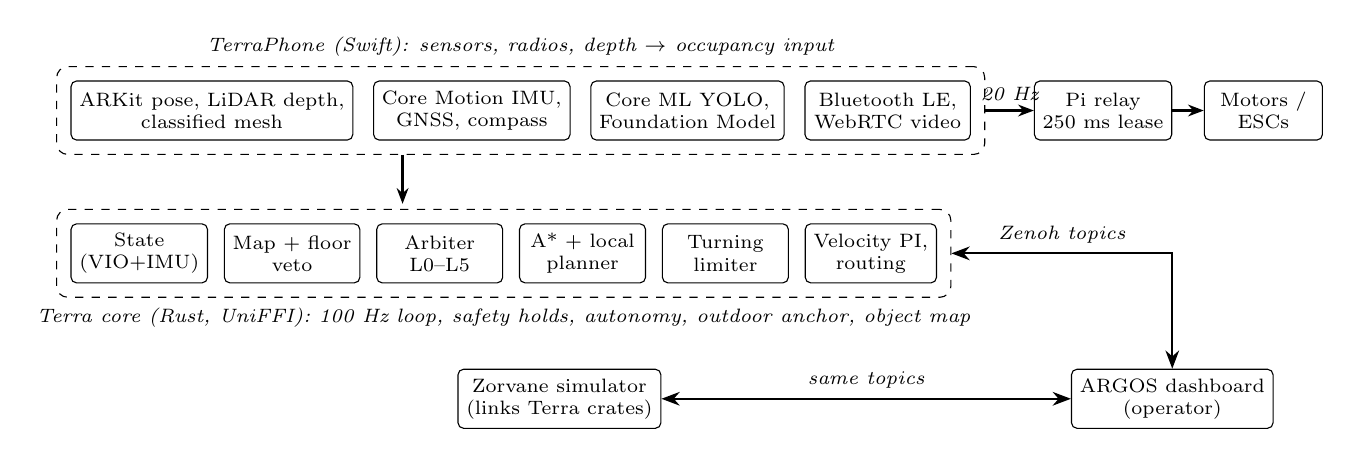
\begin{tikzpicture}[
  box/.style={draw, rounded corners=2pt, align=center, font=\scriptsize, minimum height=0.75cm, inner sep=3pt},
  grp/.style={draw, dashed, rounded corners=4pt, inner sep=5pt},
  lbl/.style={font=\scriptsize\itshape, align=center},
  edge/.style={-{Stealth[length=2mm]}, thick},
  >=Stealth]
  % Swift layer
  \node[box, minimum width=2.1cm] (ar) at (0,0) {ARKit pose, LiDAR depth,\\classified mesh};
  \node[box, minimum width=2.1cm, right=0.25cm of ar] (imu) {Core Motion IMU,\\GNSS, compass};
  \node[box, minimum width=2.1cm, right=0.25cm of imu] (yolo) {Core ML YOLO,\\Foundation Model};
  \node[box, minimum width=2.1cm, right=0.25cm of yolo] (radio) {Bluetooth LE,\\WebRTC video};
  \node[grp, fit=(ar)(radio), label={[lbl]above:TerraPhone (Swift): sensors, radios, depth $\rightarrow$ occupancy input}] (swift) {};
  % Rust core
  \node[box, minimum width=1.6cm, below=1.05cm of ar.south west, anchor=north west] (state) {State\\(VIO+IMU)};
  \node[box, minimum width=1.6cm, right=0.2cm of state] (map) {Map + floor\\veto};
  \node[box, minimum width=1.6cm, right=0.2cm of map] (arb) {Arbiter\\L0--L5};
  \node[box, minimum width=1.6cm, right=0.2cm of arb] (plan) {A* + local\\planner};
  \node[box, minimum width=1.6cm, right=0.2cm of plan] (turn) {Turning\\limiter};
  \node[box, minimum width=1.6cm, right=0.2cm of turn] (ctrl) {Velocity PI,\\routing};
  \node[grp, fit=(state)(ctrl), label={[lbl]below:Terra core (Rust, UniFFI): 100~Hz loop, safety holds, autonomy, outdoor anchor, object map}] (rust) {};
  % Pi
  \node[box, minimum width=1.6cm, right=0.8cm of radio] (pi) {Pi relay\\250~ms lease};
  \node[box, minimum width=1.5cm, right=0.4cm of pi] (motors) {Motors /\\ESCs};
  % ARGOS and Zorvane
  \node[box, minimum width=2.4cm, anchor=north] (argos) at ([yshift=-0.9cm]rust.south -| pi.east) {ARGOS dashboard\\(operator)};
  \node[box, minimum width=2.4cm, left=5.2cm of argos] (zor) {Zorvane simulator\\(links Terra crates)};
  \draw[edge] (swift.south) ++(-1.5,0) -- ++(0,-0.62);
  \draw[edge] (swift.east |- radio.east) -- node[lbl, above]{20~Hz} (pi.west);
  \draw[edge] (pi) -- (motors);
  \draw[edge, <->] (rust.east) -| node[lbl, pos=0.25, above]{Zenoh topics} (argos.north);
  \draw[edge, <->] (zor.east) -- node[lbl, above]{same topics} (argos.west);
\end{tikzpicture}
\caption{Terra architecture. Swift bridges Apple frameworks and radios; the Rust core owns the loop, safety and every autonomy level; the Pi relays wheel commands with its own lease. ARGOS talks the same Zenoh topic contract to real rovers and to Zorvane, which links the same Rust crates.}
\label{fig:arch}
\end{figure*}

Figure~\ref{fig:arch} shows the system.
The rover is a differential-drive chassis carrying an iPhone Pro with LiDAR, mounted with the rear camera facing forward, and a Raspberry Pi~4 with a motor HAT that relays wheel commands from the phone over Bluetooth Low Energy.
Two chassis share the software: a small four-motor development rover and CrabTrapBot, a roughly 0.6~m four-wheel skid-steer competition robot on which the phone sits in landscape 0.23~m above the ground.
Per-rover differences (footprint, track, speed and turn limits, motor deadband) live in a Rust \emph{rover profile}, from which the controller's feedforward gains are derived.

The phone runs TerraPhone, a Swift app of about 7{,}300 lines, over the Terra core, 17 Rust crates of about 41{,}500 lines with 399 unit tests, called through UniFFI bindings~\cite{uniffi2026}.
An Android client links the same core.
The operator station is ARGOS, a native Rust dashboard, and the simulator is Zorvane, a Bevy~\cite{bevy2026} model of the competition field that links the Terra crates directly.
All three communicate over Zenoh~\cite{zenoh2026} under one topic prefix, with one numeric identifier per rover.
\todo{State the phone model, iOS version and the cost of each chassis (phone, Pi, HAT, motors) in a bill-of-materials table.}

% ---------------------------------------------------------------------------
\section{The Swift--Rust Boundary and the Loop}
\label{sec:loop}

\subsection{One rule for splitting the code}
The project follows one rule: Swift gathers sensor data, talks to the hardware and to services that only Apple frameworks provide, and turns depth into the occupancy input; the control loop, safety gating, mode and tick policy and actuator routing belong in Rust.
The motivation is testability and reuse.
Rust code runs in the simulator and under its unit tests, so a rule that lives there is exercised in three places, whereas a rule in Swift runs only on a phone and cannot be compiled without Xcode.
The rule also makes a second platform cheap: the Android client reuses the Rust routing and control unchanged.

The split is not finished, and we report it as it stands.
The Rust step already returns the routed actuator frame, which Android sends; iOS still encodes its own frame and logs any tick where the two differ, a shadow mode that lets the Rust routing be compared with the Swift routing on real drives before it takes over.
The e-stop latch, a mount-confirmation gate and the pause on lost visual tracking still exist only in Swift.
\todo{Report the number of shadow-mode mismatches over the field runs, then the switch to the Rust frame on iOS.}

\subsection{Loop structure and freshness rules}
The loop ticks at 100~Hz.
Wheel frames go to the Pi every fifth tick, at 20~Hz, and the local planner works on a 0.1~s step.
Every stage holds when its input is stale: operator commands, maps, detector observations and the controller's target expire after 0.5~s, VIO pose after 0.35~s and IMU samples after 0.5~s, and the turning limiter holds when its step exceeds 0.1~s.
A hold clears the controller's integrators.
The Pi relay adds an independent layer: it keeps the latest command for 250~ms and then sets every output to its safe value, a zero for DC motors and a neutral pulse for ESCs; a disconnect or fault stops at once, and a battery cutoff removes motor power outright.

\subsection{Lessons: timing faults are system faults}
Freshness rules make a rover stop rather than act on old data, but on a phone they also turn any delay on the control queue into a hold.
Three faults found while building Terra were of this kind, and none was in a control law.
(i) The floor-veto mesh walk (Section~\ref{sec:map}) first ran on the control queue once a second and stalled pose and IMU delivery for about 150~ms per walk; it now runs on a utility queue.
(ii) At L3 the autonomy status carries a planner trace of about 30~KB, which the Swift tick parsed three to four times every 10~ms; one L3 run logged 191 holds for a stale IMU sample. Rust now returns a brief status under 1~KB for the hot path.
(iii) An L3 run that stalled where L2 succeeded traced to the planner's velocity window being centred on the measured speed: after a hold, a wheel inside the motor deadband measures zero, and the planner then offered at most 0.1~m/s, which kept it in the deadband. The window is now centred on the last allowed command.
Each was found because the rover records the cause of every sensor hold and ARGOS displays it.
The companion paper measures where queue delay comes from and shows that the build configuration dominates it~\cite{companion2026phone}.
The design lesson is that on a phone the platform layer's threading is part of the safety design, and that hold causes must be first-class telemetry.

% ---------------------------------------------------------------------------
\section{Mapping on a Phone}
\label{sec:map}

\subsection{Occupancy grid}
The local map is a rolling $200 \times 200$ grid of 0.1~m cells.
Each LiDAR depth pixel is back-projected, rotated into the world frame and labelled; a return between 0.15 and 2.0~m above the ground plane is an obstacle hit.
Cells along the ray are marked free and the endpoint occupied, with log-odds increments of $+0.85$ and $-0.40$ clipped to $\pm 4$, one vote per cell per frame, and a cell is occupied at $P \ge 65$.
The ground plane is level, with normal along world up, at the mount-calibrated camera height below the camera.
An earlier version used the body's up axis as the normal, and a labelled capture showed it 16$^\circ$ off gravity: floor beyond 2~m read as obstacle on one side, and walls read as free on the other.

\subsection{Floor veto from the classified mesh}
A level plane removes tilt error but not every false obstacle: depth noise, a slightly wrong camera height or a gentle slope can lift a floor return above the 0.15~m band.
ARKit also reconstructs a scene mesh and classifies its faces as floor, wall, window, door and other surfaces~\cite{apple2026arkit}, which gives an estimate of the floor independent of the depth classifier.
TerraPhone sends the centres of floor faces to the Rust map once a second.
The map bins them into 0.1~m cells, keeps the median height in each, and discards cells more than 8~cm from the median of the whole surface.
In the classifier, a return that would be an obstacle but lies less than 0.15~m above a trusted floor cell is relabelled \emph{floor veto} and clears its cell like a free return; a return higher than that above the same cell stays an obstacle, so an object on the floor is not erased.
The same surface seeds the ground-plane height when ARKit has not yet found a floor plane.
Point captures, which ARGOS can request at any time, carry the surface and the labels, so a captured frame shows exactly what the map did.
Whether a veto should count as free evidence or as no evidence, and how well ARKit classifies turf, are open; Section~\ref{sec:eval} tests both.
\todo{Report the fraction of floor returns labelled obstacle on a flat floor and on turf, with the veto on and off.}

% ---------------------------------------------------------------------------
\section{The Autonomy Ladder}
\label{sec:ladder}

\begin{table*}[t]
\centering
\caption{The Terra autonomy ladder. Every level's motion passes the same turning limiter and velocity controller and every freshness hold of Section~\ref{sec:loop}. ``GPS'' marks levels that accept a WGS84 destination.}
\label{tab:ladder}
\small
\begin{tabularx}{\textwidth}{@{}l >{\raggedright\arraybackslash}X >{\raggedright\arraybackslash}p{2.5cm} c >{\raggedright\arraybackslash}p{3.0cm}@{}}
\toprule
Level & Intent & Local planner & GPS & Operator gives \\
\midrule
L0 Teleop & Operator twist, 0.5~s lease & Bypassed & -- & Continuous drive \\
L1 Assisted & Operator twist & Chooses closest admissible command & -- & Continuous drive \\
L2 Direct & Pursuit straight to the goal & Bypassed & \checkmark & A goal \\
L3 Waypoint & Pursuit along an A* route & Checks every command & \checkmark & A goal \\
L4 Explore & Frontier with best gain per distance (toward the destination if one is set) & Checks, 1~s horizon & \checkmark & A time budget \\
L4 Search & Frontiers inside an area; detector confirmation & Checks & -- & Area, class, budget \\
L5 Task & Waypoints proposed by the on-phone model, each A*-checked & Checks & \checkmark & A typed task; answers \\
\bottomrule
\end{tabularx}
\end{table*}

\subsection{One arbiter, one planner}
All motion authority sits in one place, the arbiter in the Rust core.
Operator commands, waypoints and autonomous goals are all \emph{intents}; each level differs only in how it produces the intent $(v_i, \omega_i)$ and which layers it uses (Table~\ref{tab:ladder}).
The local planner samples an $11 \times 11$ grid of reachable twists, rolls each forward for a 2~s horizon followed by a braking tail, rejects any whose path touches an occupied, unknown or off-map cell, and picks the one closest to the intent~\cite{fox1997dwa}.
Because the braking tail is checked, an admitted command is one the rover can still stop from before anything it has seen or not seen.
When the chosen command differs from the intent, the decision is labelled \emph{assisted}, which is how ARGOS shows that the planner rather than the operator is steering.
L2 deliberately bypasses the planner so that a study can isolate the value of obstacle avoidance at L3.
L4 Explore drives to the frontier that maximises information gain per unit travel~\cite{yamauchi1997frontier}, and L4 Search runs the same explorer inside an operator-drawn rectangle while waiting for detector confirmation (Section~\ref{sec:objects}).

\subsection{A GPS destination at every level}
Outdoors the operator usually knows \emph{where} the rover should end up, not how it should get there, and GPS on a phone is too coarse, at a few metres, to avoid obstacles with.
Terra therefore treats a latitude and longitude as a \emph{final destination} that each level from L2 to L5 uses in its own way, while obstacles stay in the local VIO-frame map.
At L2 and L3 the rover follows a local target at most 3~m ahead along the geographic bearing, refreshed twice a second, at no more than 0.3~m/s; L3 routes to it with A*.
At L4 Explore the frontier score becomes $\sqrt{G}/(1 + n + 3 d_g)$ for gain $G$, travel distance $n$ and the frontier's distance $d_g$ to the destination, so exploration is pulled toward it, and GPS arrival ends the run.
At L5 the destination appears in the model's prompt as a landmark \texttt{G1}, resolved to the reachable observed point closest to it.

Two estimates join the frames.
Heading is a scalar Kalman filter on the offset between VIO yaw and true north, corrected by GPS course over ground when the rover drives straight and seeded by the compass, which near the motors read 30--50$^\circ$ off.
Position is a \emph{geographic anchor}, a 2-D Kalman filter on the rover's east and north position in which VIO travel, rotated by the fused heading, predicts and each fix corrects according to its reported accuracy; a fix more than three sigma and 3~m away is rejected, and three rejections in a row re-anchor on the newest fix.
Guidance and arrival use the smoothed position, and arrival needs three distinct fixes inside a 3~m radius.
A mission needs a fix at most 3~s old with accuracy within 10~m and heading uncertainty under 30$^\circ$; if it degrades, L2 and L3 hold while L4 and L5 withdraw the destination and keep working locally.
In the first outdoor test, with an older rule that required the arrival radius to cover the GPS accuracy, L2 stopped about 4~m short of its goal, which motivated the anchor and the 3~m radius.
\todo{Report arrival error at each level against surveyed goal points (Section~\ref{sec:eval}).}

\subsection{L5: the model proposes, Rust disposes}
At L5 the operator types a task of up to 500 characters with a time budget and a limit on model calls.
The Rust core builds a prompt from the map: the local grid reduced to 1~m symbolic cells, up to six reachable frontiers, eight obstacle blobs and eight landmarks, each with an identifier, plus the rover pose and the recent history.
Swift runs Apple's on-device Foundation Models~\cite{apple2026foundationmodels}, text only, behind a small protocol where another on-device model could be substituted.
The reply must be one JSON object choosing \texttt{go} (up to five waypoints, by identifier or as local points), \texttt{ask\_operator}, \texttt{done} or \texttt{fail}.
Rust rejects any reply that contains a speed, an effort or a servo command, snaps each waypoint to observed free space within 0.5~m, and accepts it only if A* finds a route; accepted waypoints are then driven exactly as at L3.
The model runs off the control queue and the rover holds while it thinks, so the 100~Hz tick never waits for it.
Three consecutive failed steps (invalid replies, timeouts or model errors) fail the task.
The consequence of this design is that a bad model reply costs time, not safety: everything the model can do is something an operator could already ask of L3.
\todo{L5 has not yet been run end to end on an iOS~26 phone. Report per-step model latency, reply rejection rate by reason and task completion for the fixed task set of Section~\ref{sec:eval}.}

% ---------------------------------------------------------------------------
\section{Objects on the Map}
\label{sec:objects}

The competition that motivates the fleet asks rovers to find and approach buckets, so search needs a detector.
TerraPhone runs a YOLO26n model with three classes (ball, blue bucket, orange bucket) through Core ML on the camera image, oriented by gravity rather than by the device's interface orientation so that it works with the landscape mount.
Detections are placed in the local frame using LiDAR depth.
A Rust object map merges sightings of the same class and colour within 1~m, ignores those below confidence 0.5, and confirms an object after three distinct frames; when the GPS fix is within 10~m and the heading within 35$^\circ$, it also attaches latitude and longitude.
The map is published to ARGOS, which draws confirmed objects and lists them for the operator.
L4 Search uses a stricter rule, at least three consecutive fresh observations at confidence 0.8 or more that agree within 1~m over at least 0.5~s.

In Zorvane, the same weights found most ground buckets within 10~m on their sunlit side but missed many on the shaded side (orange buckets 4 of 18 at noon, 14 of 14 overcast), found 3 of 17 buckets on 1~m stands, and gave the right colour on every detection; the median confidence of found buckets was about 0.75, below the 0.8 search threshold.
These are simulator results from parked rovers, not field results.
\todo{Measure detector recall and false positives against range and lighting on the field, and re-pick the search threshold.}

% ---------------------------------------------------------------------------
\section{Integration with ARGOS and Zorvane}
\label{sec:integration}

\paragraph{One topic contract}
Each rover publishes pose, autonomy status, hardware state, outdoor navigation and objects under its own identifier, and subscribes to level changes, goals, teleoperation and task actions.
Light telemetry is received for every rover; the occupancy grid, point clouds and depth are subscribed only for the rover the operator has selected, as CERBERUS did for camera streams~\cite{tranzatto2022finals}.
Requests that are not motion, such as a point-cloud capture, go to their own inbox outside the arbiter's authority path, and bulk replies are dropped rather than queued when the link is congested.

\paragraph{ARGOS}
ARGOS is the operator's view of the ladder: it sets levels, goals, GPS destinations, search areas and L5 tasks, and shows each rover's level, hold cause, map, video and found objects.
For the user study it can lock a rover to an assigned level and records every session to a log the experimenter can export.
\todo{One-sentence pointer to the ARGOS study paper once it exists.}

\paragraph{Zorvane}
Zorvane models the competition field at its real latitude and longitude, with CrabTrapBot as the rover, and speaks the same topics and WebRTC video as a real rover, so ARGOS cannot tell the difference.
It links Terra's state, control, mapping, navigation and autonomy crates directly, so simulated rovers run the same arbiter and levels as the phone; the phone-only parts, ARKit and the Swift layer, are replaced by simulated depth and pose.
For many rovers Zorvane runs one shared detector worker, the same YOLO weights exported to ONNX, rather than one per rover.
\todo{Quantify: how many simulated rovers run in real time on the reference laptop, and how many Terra unit tests and simulation scenarios gate a release.}

% ---------------------------------------------------------------------------
\section{Proposed Field Evaluation}
\label{sec:eval}

No field result for the ladder exists yet, so this section is a design.
It measures the system, not the sensors: VIO scale, sensor timing, GNSS accuracy and endurance are the companion paper's experiments~\cite{companion2026phone}, and runs here use the Release build that paper recommends.

\paragraph{Sites}
(S1) An indoor course in a textured hallway with three fixed obstacle layouts (open, a slalom of boxes, a doorway as narrow as the profile allows).
(S2) The motion-capture room for ground-truth paths on S1-like layouts.
(S3) The outdoor competition field, turf, with surveyed goal points.
\todo{Confirm S3 access and how goal points will be surveyed (RTK GNSS or tape from a landmark).}

\paragraph{Experiments}
Table~\ref{tab:eval} lists the experiments.
Each run records the Terra observability journal and the ARGOS session log, which together give level, intent, chosen command, hold cause and objects at every tick.

\begin{table*}[t]
\centering
\caption{Proposed field experiments. Every result cell in the paper stays \todo{} until the run is done.}
\label{tab:eval}
\small
\begin{tabularx}{\textwidth}{@{}l >{\raggedright\arraybackslash}p{4.0cm} >{\raggedright\arraybackslash}X >{\raggedright\arraybackslash}p{3.3cm}@{}}
\toprule
ID & Question & Protocol & Metrics \\
\midrule
F1 & Does each level reach goals, and at what cost in operator input? & S1 and S3; L0--L3 to the same goal, 10 runs per level per layout, randomized order; trained operator & Success, time, path length ratio, collisions, operator inputs, holds by cause \\
F2 & Does the floor veto remove false obstacles without hiding real ones? & S1 floor and S3 turf; Capture 3D with veto on and off; L3 runs through the slalom with each & Floor returns labelled obstacle; missed boxes; L3 success and clearance \\
F3 & How close does each level get to a GPS destination? & S3; 5 surveyed goals 20--80~m away; L2, L3, L4 and L5 with a GPS destination, 5 runs each & Arrival error, time, pauses and re-anchors, success \\
F4 & Can L4 find buckets on the field? & S3; buckets on the ground and on stands, sun and shade; L4 Search, 10 runs & Time to confirm, recall, false objects, geotag error \\
F5 & Does L5 complete simple tasks safely? & S1 then S3; a fixed set of 5 typed tasks, 5 runs each & Completion, model calls, per-step latency, rejected replies by reason, operator questions \\
F6 & Does simulation predict the field? & Repeat F1 and F4 layouts in Zorvane & Difference in success and time between sim and field \\
F7 & Does the loop keep up in the field? & All runs & Tick rate, holds per minute by cause, shadow-mode mismatches, phone temperature state \\
\bottomrule
\end{tabularx}
\end{table*}

\paragraph{Analysis}
F1 compares levels with a mixed model with layout as a random effect; F2 reports the false-obstacle fraction with and without the veto and a paired comparison of L3 success; F3 reports median and 95th-percentile arrival error per level.
\todo{Fix the number of runs per cell after a pilot day; the counts above are placeholders sized for a two-day campaign.}

\paragraph{Results}
\todo{Table: F1 success and time per level and layout.}
\todo{Figure: F2 point captures with veto off and on.}
\todo{Table: F3 arrival error per level.}
\todo{F4--F7 results.}

% ---------------------------------------------------------------------------
\section{Discussion and Limitations}
\label{sec:discussion}

\paragraph{What the phone changes}
The phone gives a rover depth, a pose estimate, GNSS, a camera, a neural accelerator and radios for the price of a handset, but it brings an operating system that owns the threads, the thermal limits and the build configuration.
The faults in Section~\ref{sec:loop} came from there, not from the control laws, and the fix each time was to move work out of the platform layer or off its control queue.
This is the strongest argument for the Swift--Rust rule: the less the platform layer decides, the less of the rover's behaviour depends on the platform's scheduler.

\paragraph{Limitations}
The system has been tested indoors and in short outdoor runs, not in the campaign of Section~\ref{sec:eval}.
The floor veto and the L5 runner were merged without a device build at the time, and L5 has not completed a task end to end.
VIO under-reads distance by about 9\% in our motion-capture room~\cite{companion2026phone}; the rover stays consistent with its own map, but absolute distances and GPS goals inherit the error.
LiDAR sees through glass, and a barrier label from the classified mesh did not stop the rover at real glass in a first test.
Arming is not yet enforced in the Rust core: the relay keeps only a lease, and the e-stop latch is still in Swift.
\todo{Update each limitation after the field campaign.}

% ---------------------------------------------------------------------------
\section{Conclusion}
\label{sec:conclusion}

Terra shows that a consumer phone can carry a complete, layered autonomy stack for a small rover, and that splitting the software so that a shared Rust core owns control, safety and autonomy makes the same stack run on the phone, in simulation and under a remote operator.
On that core, a six-level ladder gives an operator a choice from direct driving to typed tasks, with a GPS destination at every level that moves and a language model that can only propose where to go.
\todo{Close with the headline field result.}

\section*{Acknowledgment}
\todo{Advisor, lab members (dumper, basestation, YOLO training, map fusion), funding.}

\bibliographystyle{IEEEtran}
\bibliography{references}

\end{document}
